\subsection{Dark matter and its connection to antinuclei}

\subsubsection{The evidence for dark matter}
\subsubsection{WIMP dark matter and the WIMP miracle}\label{sec:IntroWIMPs}
The WIMP miracle is well known to be the fact that when one considers a particle of the weak mass scale with a self annihilation cross section close to the weak interaction strength (on the pb level), the present day dark matter relic density can be obtained. Additionally, in many versions of supersymmetry, the lightest supersummetric particle is indeed a weakly interacting heavy particle, the ideal scenario for the WIMP\cite{}. In the following section the derivation of the WIMP abundance is shown, which is reproduced here from \cite{Baer-Choi-Kim}. The WIMP is denoted as $\chi$, and it is assumed be in thermal equilibrium with other matter while the Temperature is $T>$\dmm . During this time, the WIMP density $n_\chi$ evolves according to the Boltzmann equation, shown in equation \ref{eq:boltzman_deriv_eq}: 
\begin{equation}\label{eq:boltzman_deriv_eq}
    \frac{dn_\chi}{dt} = -3H n_\chi - <\sigma_{ann}v>(n_\chi^2 - n_{eq}^2)
\end{equation}
where H is the Hubble constant at that time, which in a radiation dominated universe is given by $H^2 = \rho_{rad}/3M^2_P$, where $M_P$ is the plank mass. While the system is in equilibrium, the number density tracks the equilibrium density $n_{eq}$. Subsequently, at some temperature $T_f$<m$_\chi$, the expansion rate will exceed the annihilation rate, and dark matter will freeze out, and their comoving number density (i.e. the number density accounting for the volumetric expansion of the universe) will remain constant from this point on. An approximate solution to the Boltzmann equation at this point gives equation \ref{eq:sol_Boltzmann}, where $\Omega_\chi h^2$ is the dimensionless dark matter density in the universe\footnote{$\Omega_\chi$ can be interpreted as the curvature of space which dark matter is responsible for.}, $s_0$ is the present day entropy density of the Universe, $g_*$ is the number of relativistic degrees of freedom of the particle $\chi$ at freeze out, and $x_f = T_f/m_\chi \approxeq 1/25$ is the freeze out temperature scaled to the dark matter mass. The value for $x_f=1/25$ is obtained from solving the Friedmann equation\footnote{This is the solution to Einstein's field equations for an open, closed or flat universe.} numerically for the freezeout Temperature (see \ref{Baer} for more details). This means that WIMPs would have still moved at relativistic speeds at freezeout, with velocities $<v>\approx c/3$. 

\begin{equation}
    \label{eq:sol_Boltzmann}
    \Omega_\chi h^2 \approx \frac{s_0}{\rho_c/h^2} \left( \frac{45}{\pi^2g_*}\right)^2 \frac{1}{x_f M_P} \frac{1}{<\sigma_{ann}v>}
\end{equation}

Plugging in the known values for the parameters\cite{ref 533 DM review} and setting $\Omega_\chi h^2$ = 0.12 from the latest Planck Collaboration results \cite{Planck2018}, one obtains equation \ref{eq:DM_relic_density}. 

\begin{equation}
    \label{eq:DM_relic_density}
    \frac{\Omega h^2}{0.12} = \frac{1}{<\frac{\sigma_{ann}}{10^{-36} cm^2} \frac{v/c}{0.1}}
\end{equation}

Thus, setting the thermally averaged annihilation cross section to a value of 1pb * $c$, and using average velocities of the order one would expect from a WIMP at freezeout, the current dark matter abundance is recovered. A schematic representation of this process is shown in figure \ref{fig:DM_thremal_eq_freeze_out}, where the decoupling temperature $T_{dec}$ and the freezeout temperature $T_{f}$ are shown separately. The decoupling temperature is the temperature at which the dark matter and luminous matter stop being in thermal equilibrium, while the freeze out temperature the point where the expansion rate becomes the dominant term for the density change for dark matter, over the annihilation term. 

\begin{figure}[htbp]
    \centering
    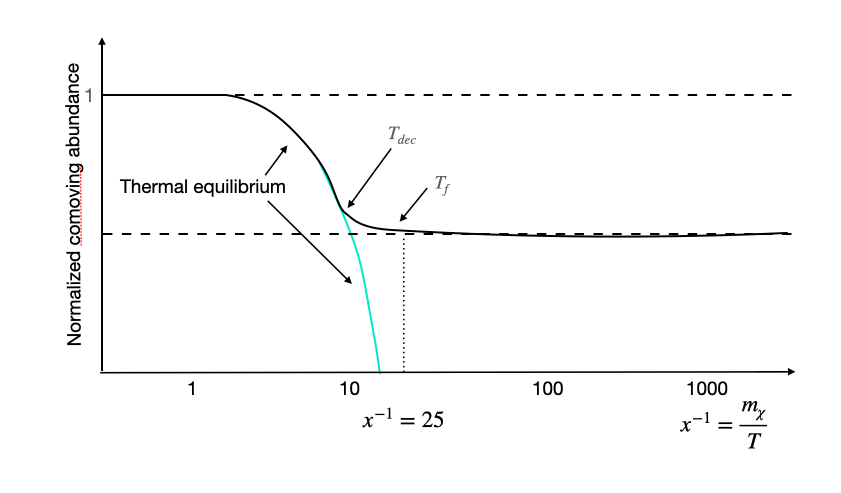
\includegraphics[width=\textwidth]{figures/schematic_thermal_eq_evolution_DM.png}
    \caption{Transition of dark matter from thermal equilibrium to freeze out. Both the decoupling temperature (where dark matter stops being in thermal equilibrium with luminous matter) and the freeze out temperature (when the rate of expansion has dropped the annihilation rate to negligible amounts, so that the comoving density can be considered constant) are indicated on the schematic. Figure is based on the figure in \cite{Baer}}
    \label{fig:DM_thremal_eq_freeze_out}
\end{figure}



\subsubsection{Other dark matter models}\label{IntroOtherDM}
\subsubsection{Dark matter annihilations into antinuclei}
\subsubsection{Majorana vs. Dirac dark matter}\label{sec:IntroMajoranaDiracDM}
Since the properties of dark matter are not know beyond its gravitational pull, it is also not known if dark matter is its own anti-particle. 
\subsubsection{Thermal self-annihilation cross section in the early universe}
\subsubsection{The distribution of dark matter within our galaxy}
\subsubsection{The search for dark matter: the link between WIMP dark matter and antinuclei}